\subsection{Winston cones refurbishment}

Winston Cones (WC) are used to collect light onto the PMTs. In the LTCC there are three kind of WC:

\begin{enumerate}

\item Small
	\begin{enumerate}
		\item Height: 18cm
		\item Parallel Plate distance: 14cm
		\item Radius at the top: 20cm
		\item Radius at the bottom: 11cm
		\item Material: copper (electro-formed)
	\end{enumerate}

	\item Medium
	\begin{enumerate}
		\item Height: 22cm
		\item Parallel Plate distance: 15cm
		\item Radius at the top: 20cm
		\item Radius at the bottom: 11cm
		\item Material: 0.2” plastic (vacuum pressed)
	\end{enumerate}

	\item Large
	\begin{enumerate}
		\item Height: 30cm
		\item Parallel Plate distance: 18cm
		\item Radius at the top: 22cm
		\item Radius at the bottom: 11cm
		\item Material: copper (electro-formed)
	\end{enumerate}
\end{enumerate}

The reflectivity of the WC showed the same degradation as 
A setup on an optical bench allowed to measure the reflectivity for all the WCs at wavelengths between 200 and 400 nm was designed to accept incident light
shallow angles of 10-15 degrees (typical incident angle based on simulation studies), see \F{wcSetup}. A typical reflectivity of a poor WC is shown in \F{wcStatusBefore} (top).
All 216 WC were measured, and the results are shown in \F{wcStatusBefore} (bottom). This allowed to catalog the quality of the WC, as the

\begin{figure}
	\centering
	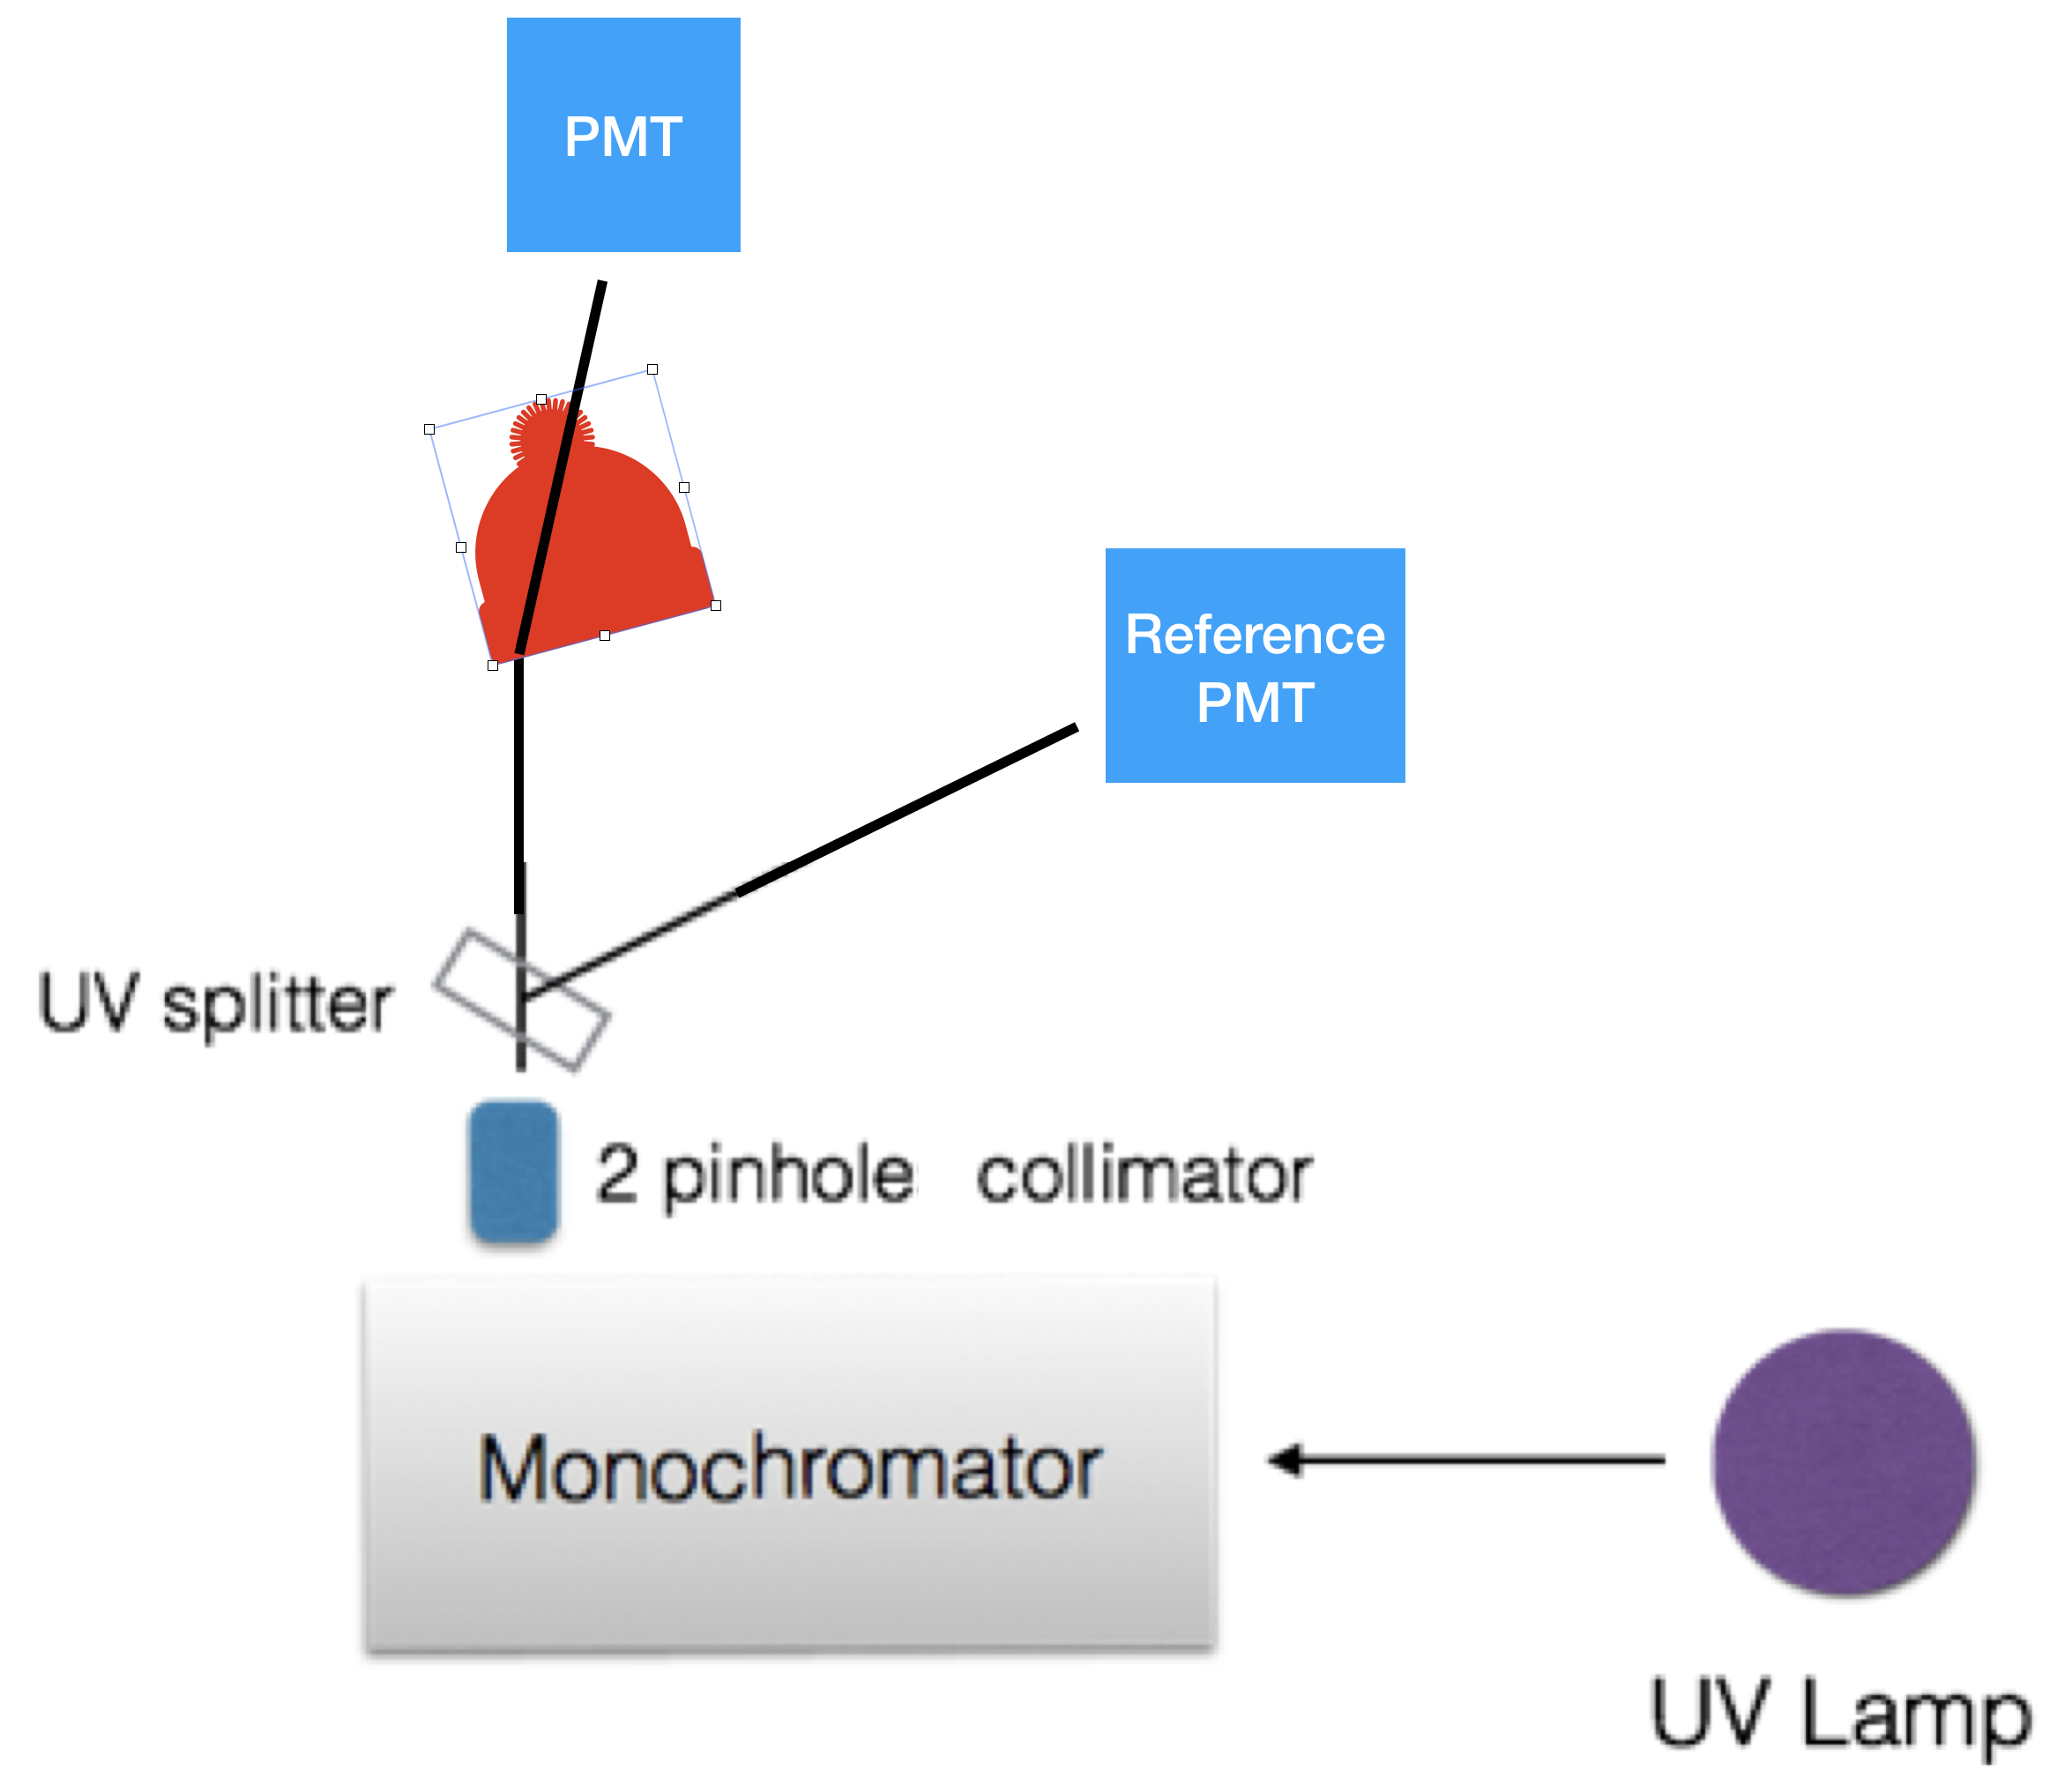
\includegraphics[width=0.95\columnwidth,keepaspectratio]{img/wcSetup.png}
	\caption{Setup to measure the WC reflectivity. The wavelength of light from a deuterium lamp was measured using a mono-chromator and splitted in two
            light beams, each with calibrated intensity. One of the light beam impinged on the WC at a typical angle of 12 degrees, while the other was directed at the reference PMT.
				}
	\label{fig:wcSetup}
\end{figure}


\begin{figure}
	\centering
	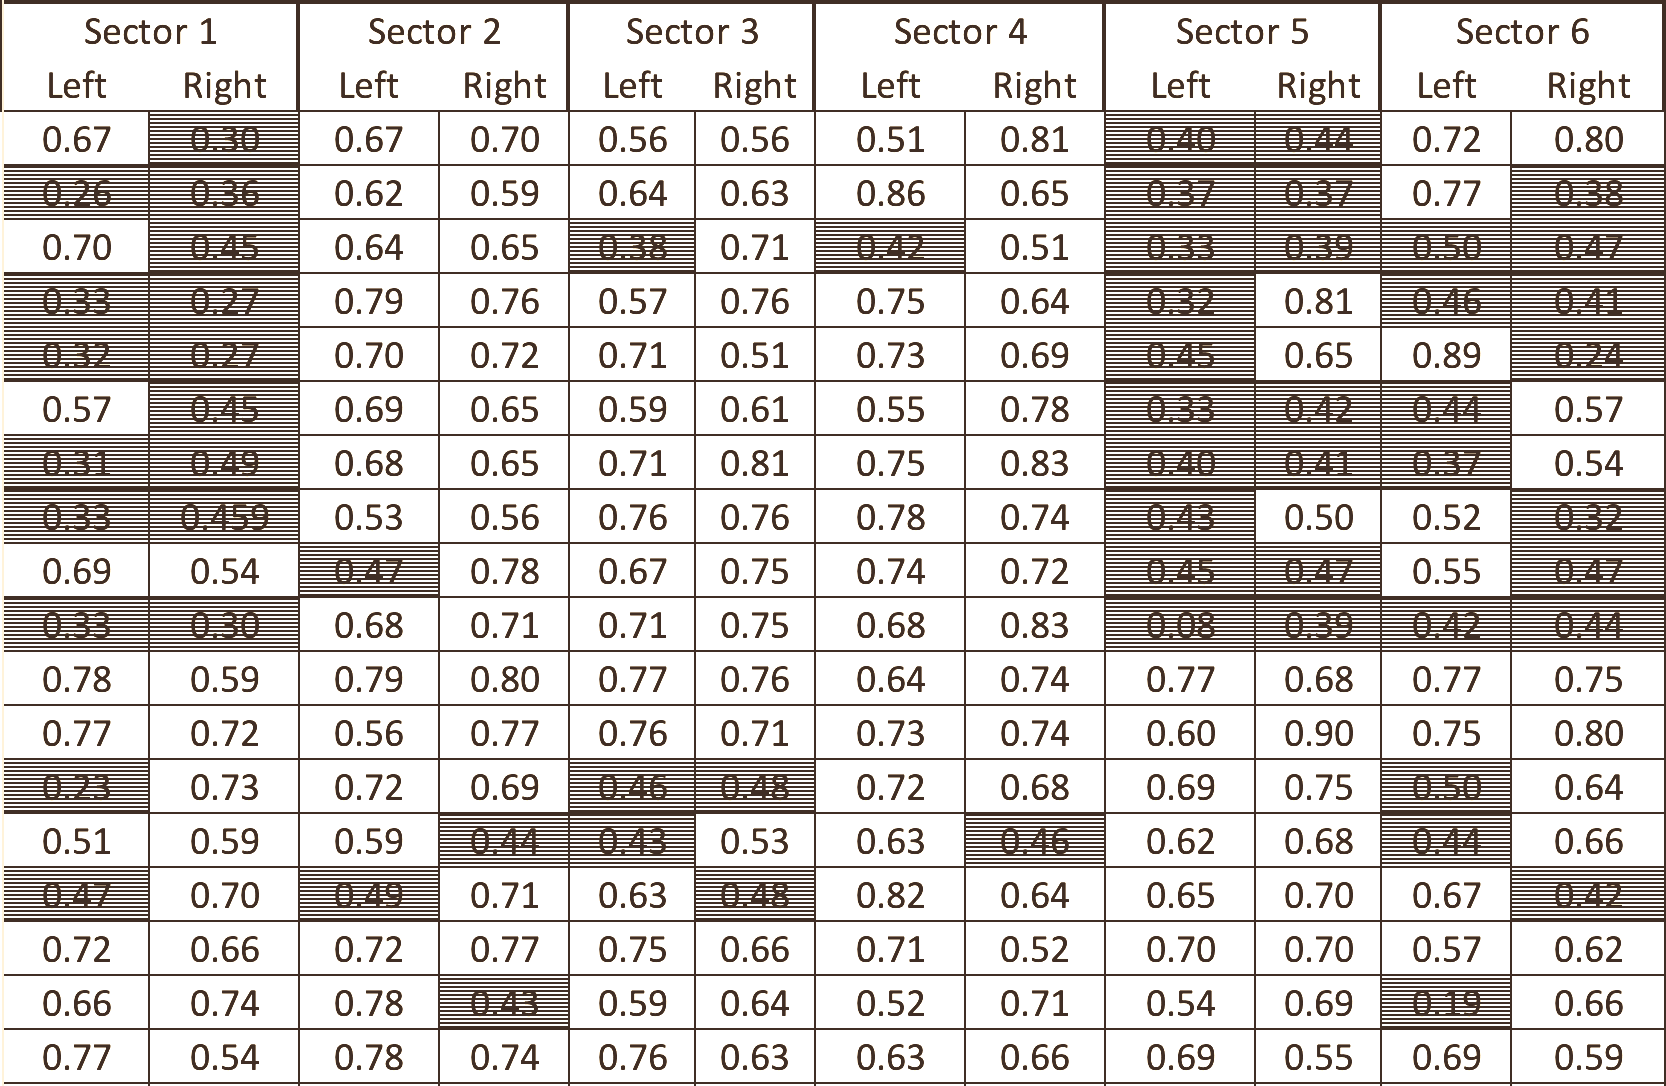
\includegraphics[width=1.0\columnwidth,keepaspectratio]{img/wcStatusBefore.png}
	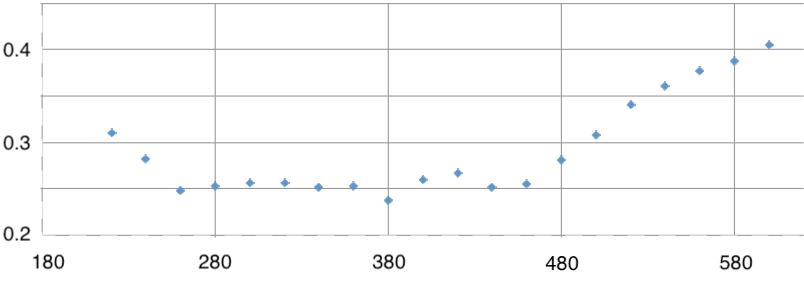
\includegraphics[width=1.0\columnwidth,keepaspectratio]{img/winstoConeSample2Reflectivity.png}
\caption{Top: typical reflectivity of a poor WC.  }
	\label{fig:wcStatusBefore}
\end{figure}


\begin{figure}
	\centering
	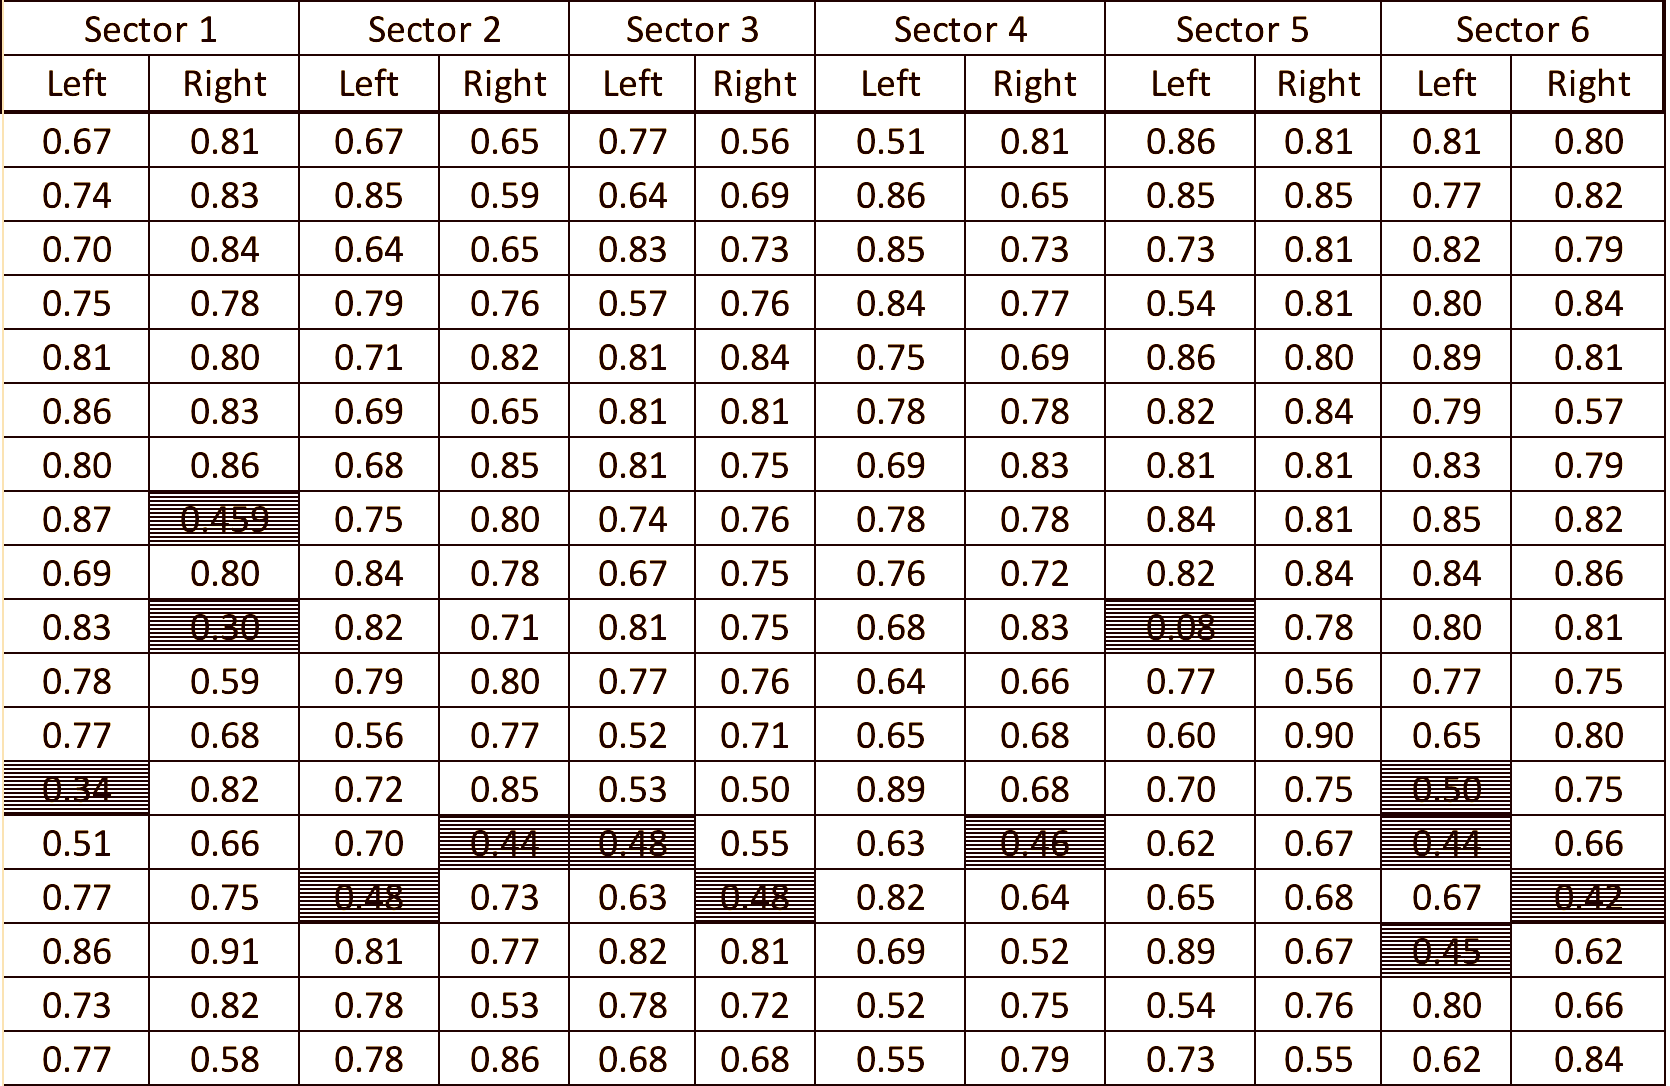
\includegraphics[width=1.0\columnwidth,keepaspectratio]{img/wcStatusAfter.png}
	\caption{Top view of the back-wall of the LTCC. A stainless steel bar encapsulate a sandwich wall of aluminum and foam. On the left and right side
			of the frame a new patch panel allow for 3 hermetical connectors (1 HV, 2 signals) from each PTM. }
	\label{fig:wcStatusAfter}
\end{figure}

\begin{figure}
	\centering
	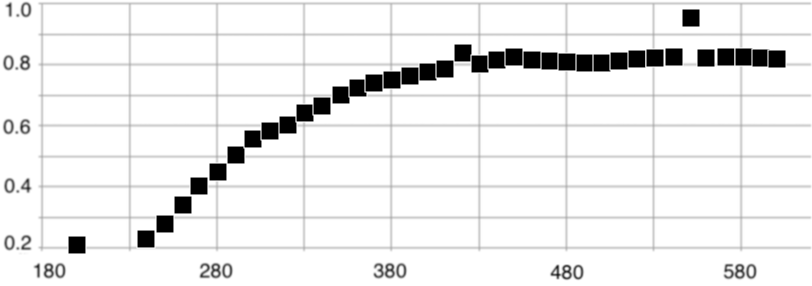
\includegraphics[width=1.0\columnwidth,keepaspectratio]{img/winstoConeSample1Reflectivity.png}
	\caption{Top view of the back-wall of the LTCC. A stainless steel bar encapsulate a sandwich wall of aluminum and foam. On the left and right side
			of the frame a new patch panel allow for 3 hermetical connectors (1 HV, 2 signals) from each PTM. }
	\label{fig:wcReflectivitySamples}
\end{figure}

